
\documentclass[11pt,letterpaper]{article}

% Load some basic packages that are useful to have
% and that should be part of any LaTeX installation.
%
% be able to include figures
\usepackage{graphicx}
% get nice colors
\usepackage{xcolor}

% change default font to Palatino (looks nicer!)
\usepackage[latin1]{inputenc}
\usepackage{mathpazo}
\usepackage[T1]{fontenc}
% load some useful math symbols/fonts
\usepackage{latexsym,amsfonts,amsmath,amssymb}

% comfort package to easily set margins
\usepackage[top=1in, bottom=1in, left=1in, right=1in]{geometry}

% control some spacings
%
% spacing after a paragraph
\setlength{\parskip}{.15cm}
% indentation at the top of a new paragraph
\setlength{\parindent}{0.0cm}


\begin{document}

\begin{center}
\Large
Ay190 -- Worksheet 6\\
Anthony Alvarez\\
Date: January 30, 2014
\end{center}

\section{The Discrete Forier transform of a vector }
\subsection{Correctness}

When comparring the function that I wrote dft() to the numpy version of dft 
fft() I find that the results are equivalent to within $0.00000001$. That is 
close enough and I would say that the results are equal.

\subsection{Timing}

While I have shown that I \textit{can} use my own implementation of dft
it is generaly a good idea to check for packages which are already written
as they are usually much faster. As we can see in figure~\ref{fig:dft} my dft
implementation is absolutely much slower and also has worse scaling proporties
when compared with the numpy version. 

\begin{figure}[bth]
\centering
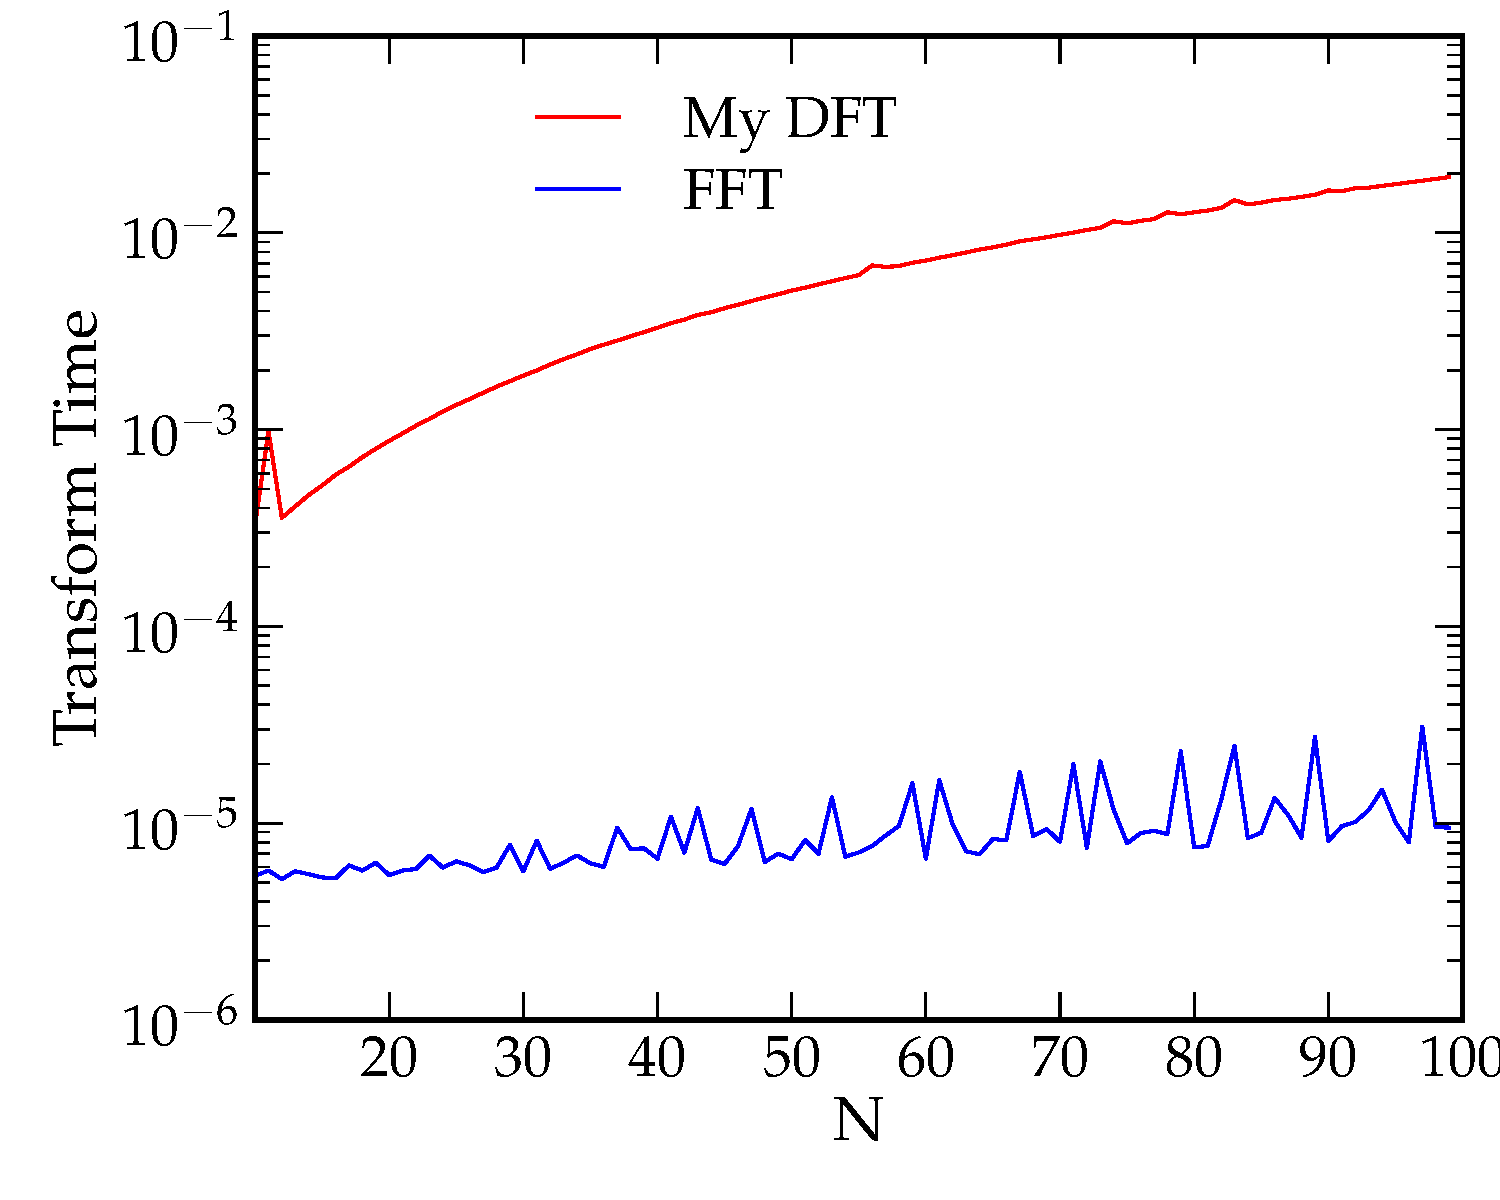
\includegraphics[width=0.5\textwidth]{1b.pdf}
\caption{My DFT runs much less efficiently than the numpy FFT. Both running 
absolutely slower and having worse scalling proporties.}
\label{fig:dft}
\end{figure}


\end{document}




